\chapter{Конструкторская часть}

\section{Требования к программному обеспечению}

К разрабатываемому программному обеспечению предъявляются следующие 5 требований:
\begin{enumerate}
  \item ввод размера массива $N$ (натуральное число);
  \item автоматическое наполнение массива $A$ $N$ уникальными целочисленными значениями;
  \item создание дубликата массива $A$;
  \item сортировка элементов дубликата по возрастанию;
  \item циклический вывод интерактивного меню с возможностью выбора и выполнения следующих операций:
  	\begin{itemize}
  		\item вывод отсортированного дубликата массива $A$;
  		\item выбор используемого алгоритма поиска;
      	\item ввод искомого значения $x \in \mathbb{Z}$;
      	\item вывод индекса элемента, равного $x$, или $-1$, если элемент отсутствует;
      	\item выход из программы.
    \end{itemize}
\end{enumerate}

\section{Разработка алгоритмов}
Для каждого алгоритма определены:
\begin{itemize}
	\item $A$ --- входной массив уникальных целых чисел;
	\item $N$ --- количество элементов массива $A$;
	\item $x$ --- искомый элемент;
	\item $index$ --- индекс найденного элемента внутри массива $A$ (значение $-1$ при отсутствии).
\end{itemize}

Для алгоритмов бинарного поиска дополнительно определено:
\begin{itemize}
	\item $l$ --- индекс левой границы обрабатываемой части массива $A$;
	\item $r$ --- индекс правой границы обрабатываемой части массива $A$;
	\item $m$ --- индекс серединного элемента обрабатываемой части массива $A$.
\end{itemize}

\subsection{Поиск полным перебором}
При алгоритме поиска полным перебором в массиве $A$ последовательно перебираются его элементы от индекса $0$ до $N − 1$ и сравниваются с искомым значением. При совпадении поиск завершается с результатом --- индексом найденного элемента. В случае перебора всех элементов массива и отсутствии совпадения результат приравнивается к $-1$. 
Схема алгоритма приведена на рисунке~\ref{img:algo-brute-force}.
\begin{figure}[H]
	\centering
	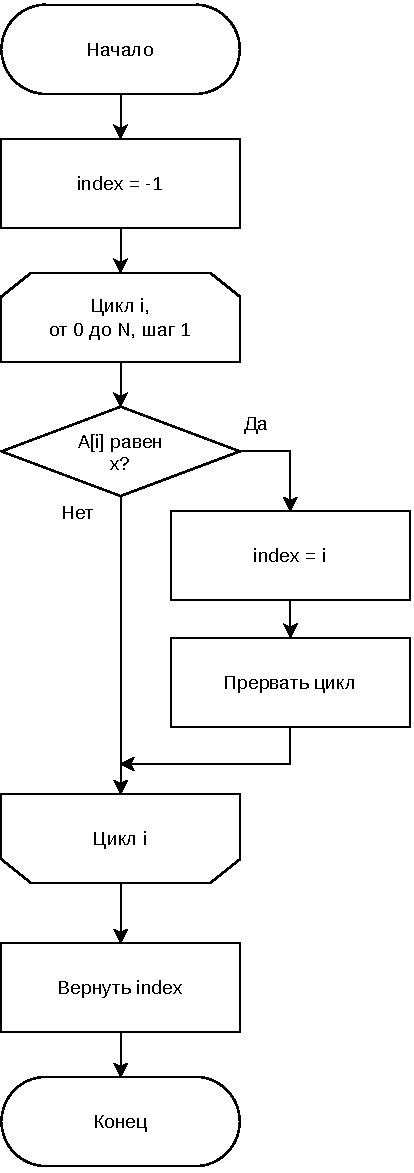
\includegraphics[scale=0.9]{image/algo/algo_1.pdf}
	\caption{Схема алгоритма поиска полным перебором}
	\label{img:algo-brute-force}
\end{figure}

\subsection{Нерекурсивный бинарный поиск}
При нерекурсивной реализации алгоритма бинарного поиска рассматривается массив, отсортированный по возрастанию. Вводятся переменные, обозначающие границы обрабатываемой части массива. Изначально $l = 0$, $r = N - 1$. На каждой итерации цикла внутри поиска определяется средний элемент массива с индексом $m = l + (r - l) / 2$. Для следующей итерации определяются новые границы обрабатываемой части массива с помощью сравнения среднего элемента с искомым значением. 

Поиск продолжается до тех пор, пока $l < r$. После завершения цикла элемент $A[l]$ сравнивается с искомым: при совпадении результатом поиска является индекс $l$, иначе искомый элемент в массиве отсутствует.

Схемы нерекурсивных алгоритмов бинарного поиска приведены на рисунках~\ref{img:algo-bin-search-1} и~\ref{img:algo-bin-search-2}.

\begin{figure}[H]
	\centering
	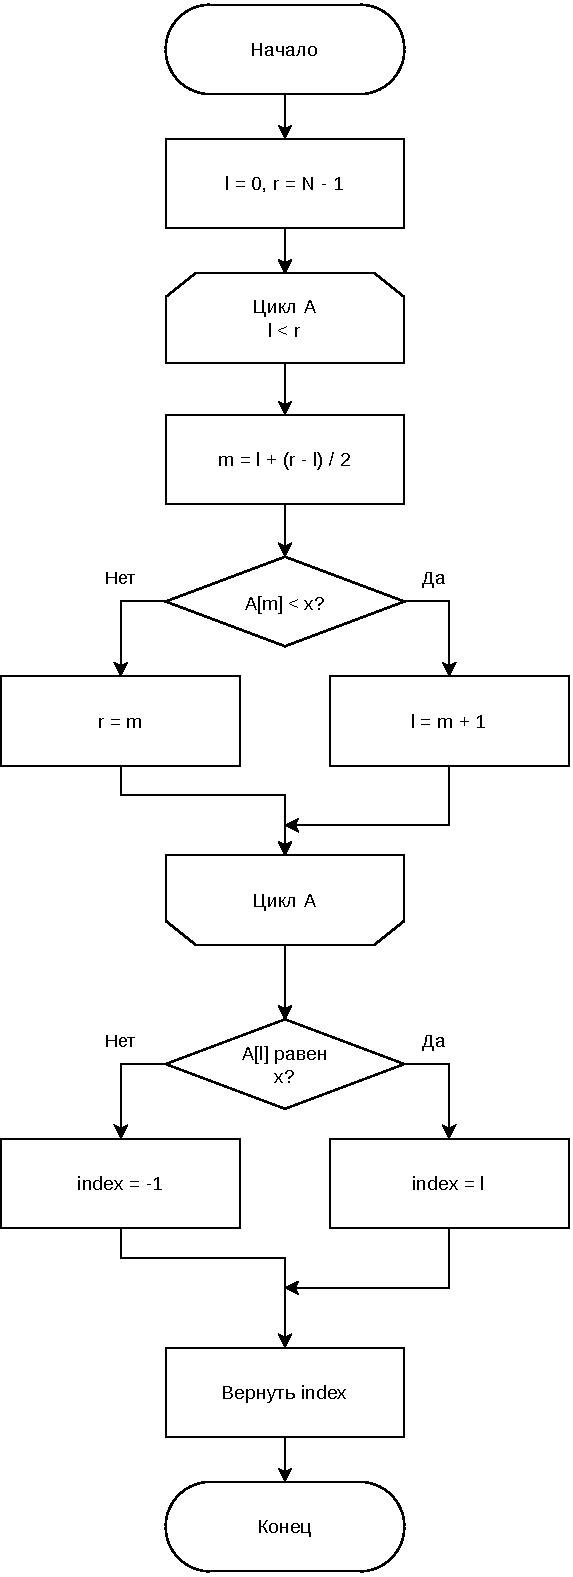
\includegraphics[scale=0.9]{image/algo/algo_2.pdf}
	\caption{Схема нерекурсивного алгоритма бинарного поиска с отложенным выходом}
	\label{img:algo-bin-search-1}
\end{figure}

\begin{figure}[H]
	\centering
	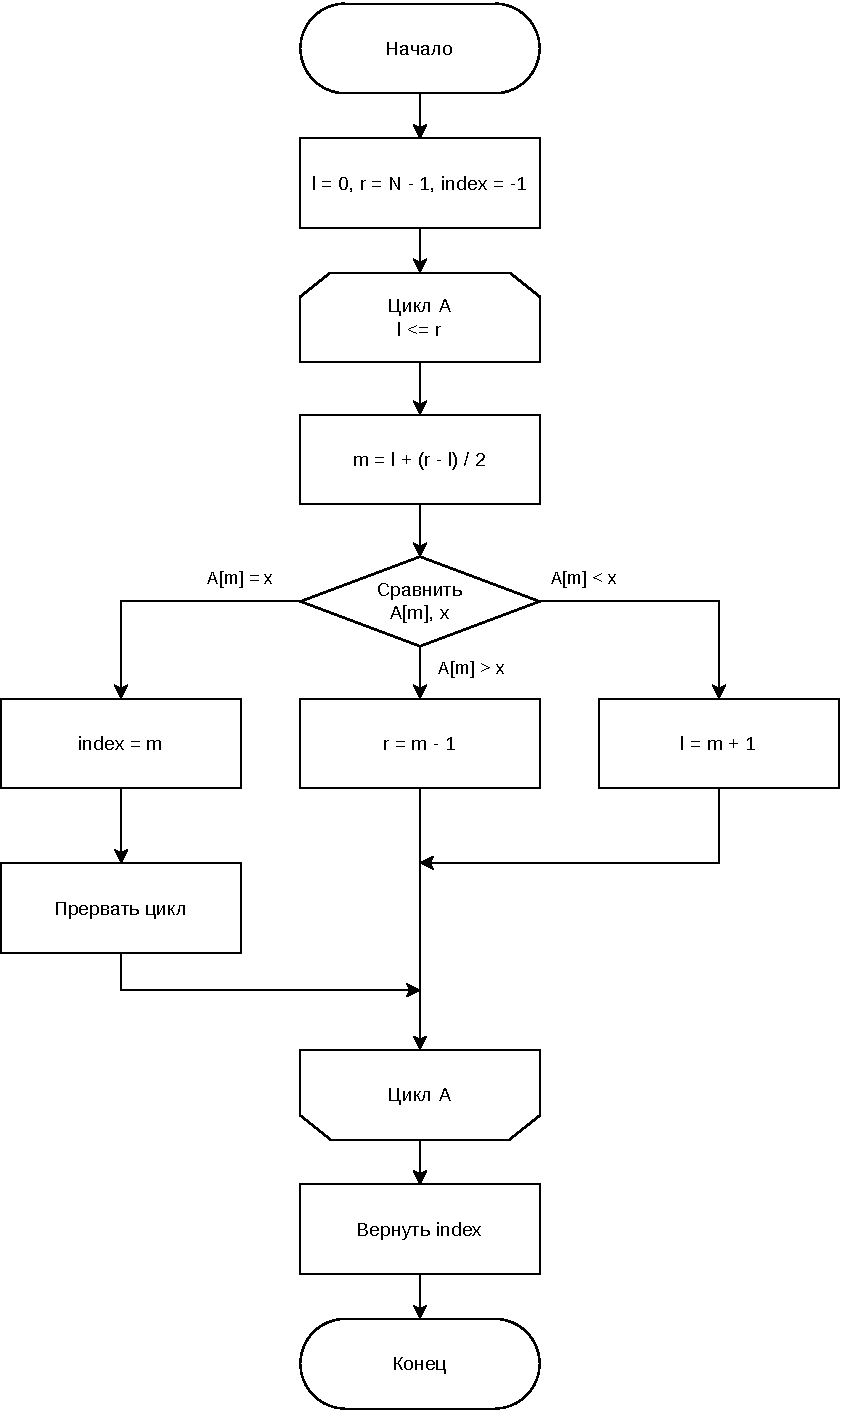
\includegraphics[scale=0.9]{image/algo/algo_3.pdf}
	\caption{Схема нерекурсивного алгоритма бинарного поиска с предварительным выходом}
	\label{img:algo-bin-search-2}
\end{figure}

\subsection{Рекурсивный бинарный поиск}
При рекурсивной реализации алгоритма бинарного поиска реализуется аналогичный принцип деления обрабатываемой части массива пополам, что и нерекурсивные реализации, однако организуется рекурсивный вызов функции с новыми границами обрабатываемой части.
На рисунке~\ref{img:algo-bin-search-r} представлена схема рекурсивной процедуры бинарного поиска.

\begin{figure}[H]
	\centering
	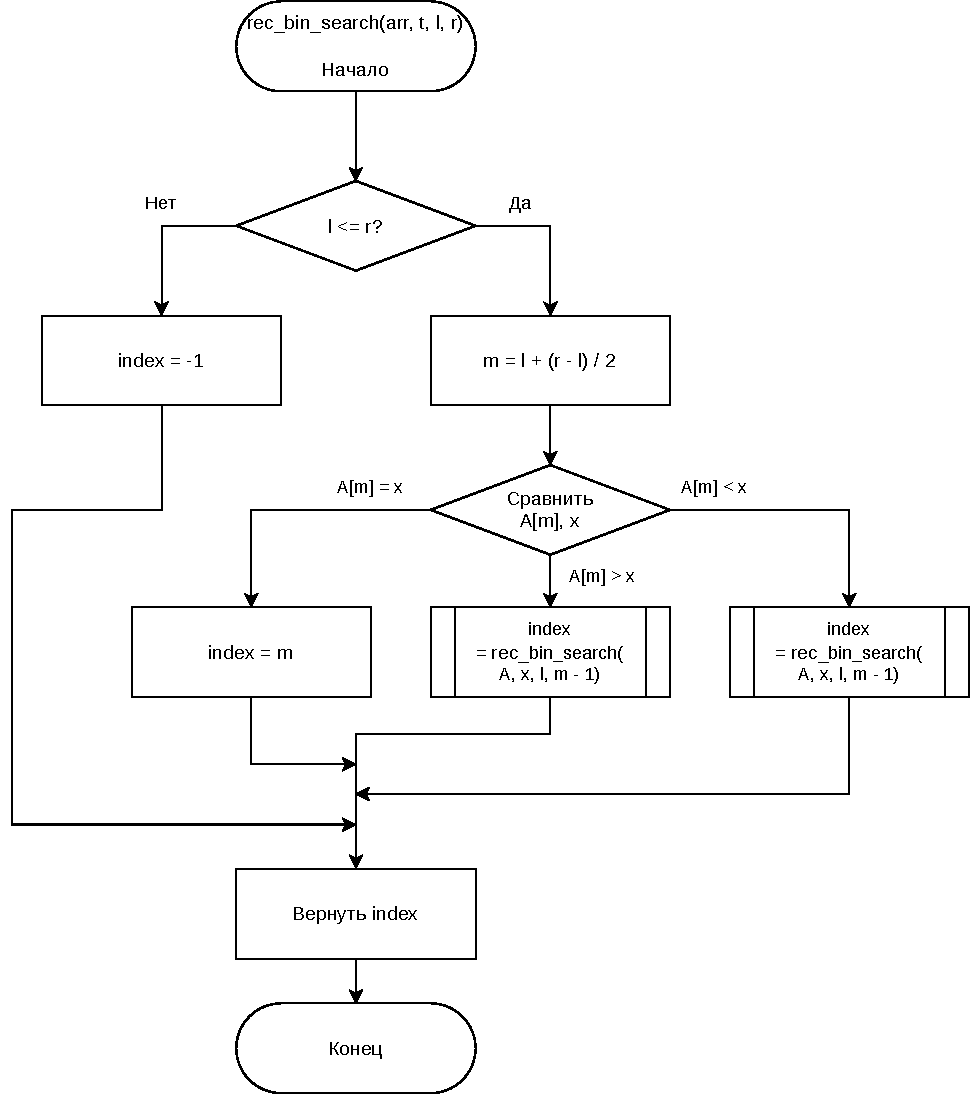
\includegraphics[scale=0.9]{image/algo/algo_4.pdf}
	\caption{Схема рекурсивного алгоритма бинарного поиска}
	\label{img:algo-bin-search-r}
\end{figure}

\section{Вывод}
В результате конструкторской части были определены требования к программному обеспечению, были описаны с помощью схем алгоритмов варианты реализации алгоритма поиска элемента в массиве.